\subsection{Music recommendation}
Collaborative filtering is the part of recommender systems that predicts users' preferences for particular items. The major challenge in predicting users'listening count, as in our task, is that the available user-artist counts are usually too few and sometimes a method's performance relies on a good initial estimation of the unknown entries. 
These are reasons why we decided to implement besides the common Kmeans, KNN also ALS[cite here], which uses only the known listening counts and avoids dependency on initial estimations.

\subsection{Data description}
The training data consists in a matrix $Ytrain$ of size $1774x15082$, corresponding to $1774$ users and $15802$ artists. Element $Ytrain(i,j)$ expresses how many times user i has listened to artist j. An entry of 0 means we do not have information for that (user, artist, count) triple.
We are also given the friendship graph of the $1774$ users stored as an adjacency matrix.

\subsection{Exploratory Data Analysis}

The listening counts matrix is very sparse with a density of only $0.0026\%$, corresponding to 
$69617$ (user, artist, count) triples.
The highest count is $352698$, the average listening count per user is  5.52 and the average listening count per artist is 5.46 but the variance is very high.
A histogram of all the listening counts, shown in Fig\ref{fig:count_distribution} tells us that the listening counts follow a heavy tail distribution. The long tail contains a small number of popular items, the well-known
artists, and the rest are located in the heavy tail.
One method to transform skewed data such that it becomes more gaussian distributed is to use the Box-Cox transform[cite]. In our case, we can choose $\lambda=0$ since for us  y values are very high and positive. This transformation will make the distances between listening counts much smaller and will reduce the influence on RMSE of the (user,artist,count) triples in the long tail. 

\begin{figure}[h]
  \centering
  \begin{subfigure}[b]{0.45\textwidth}
   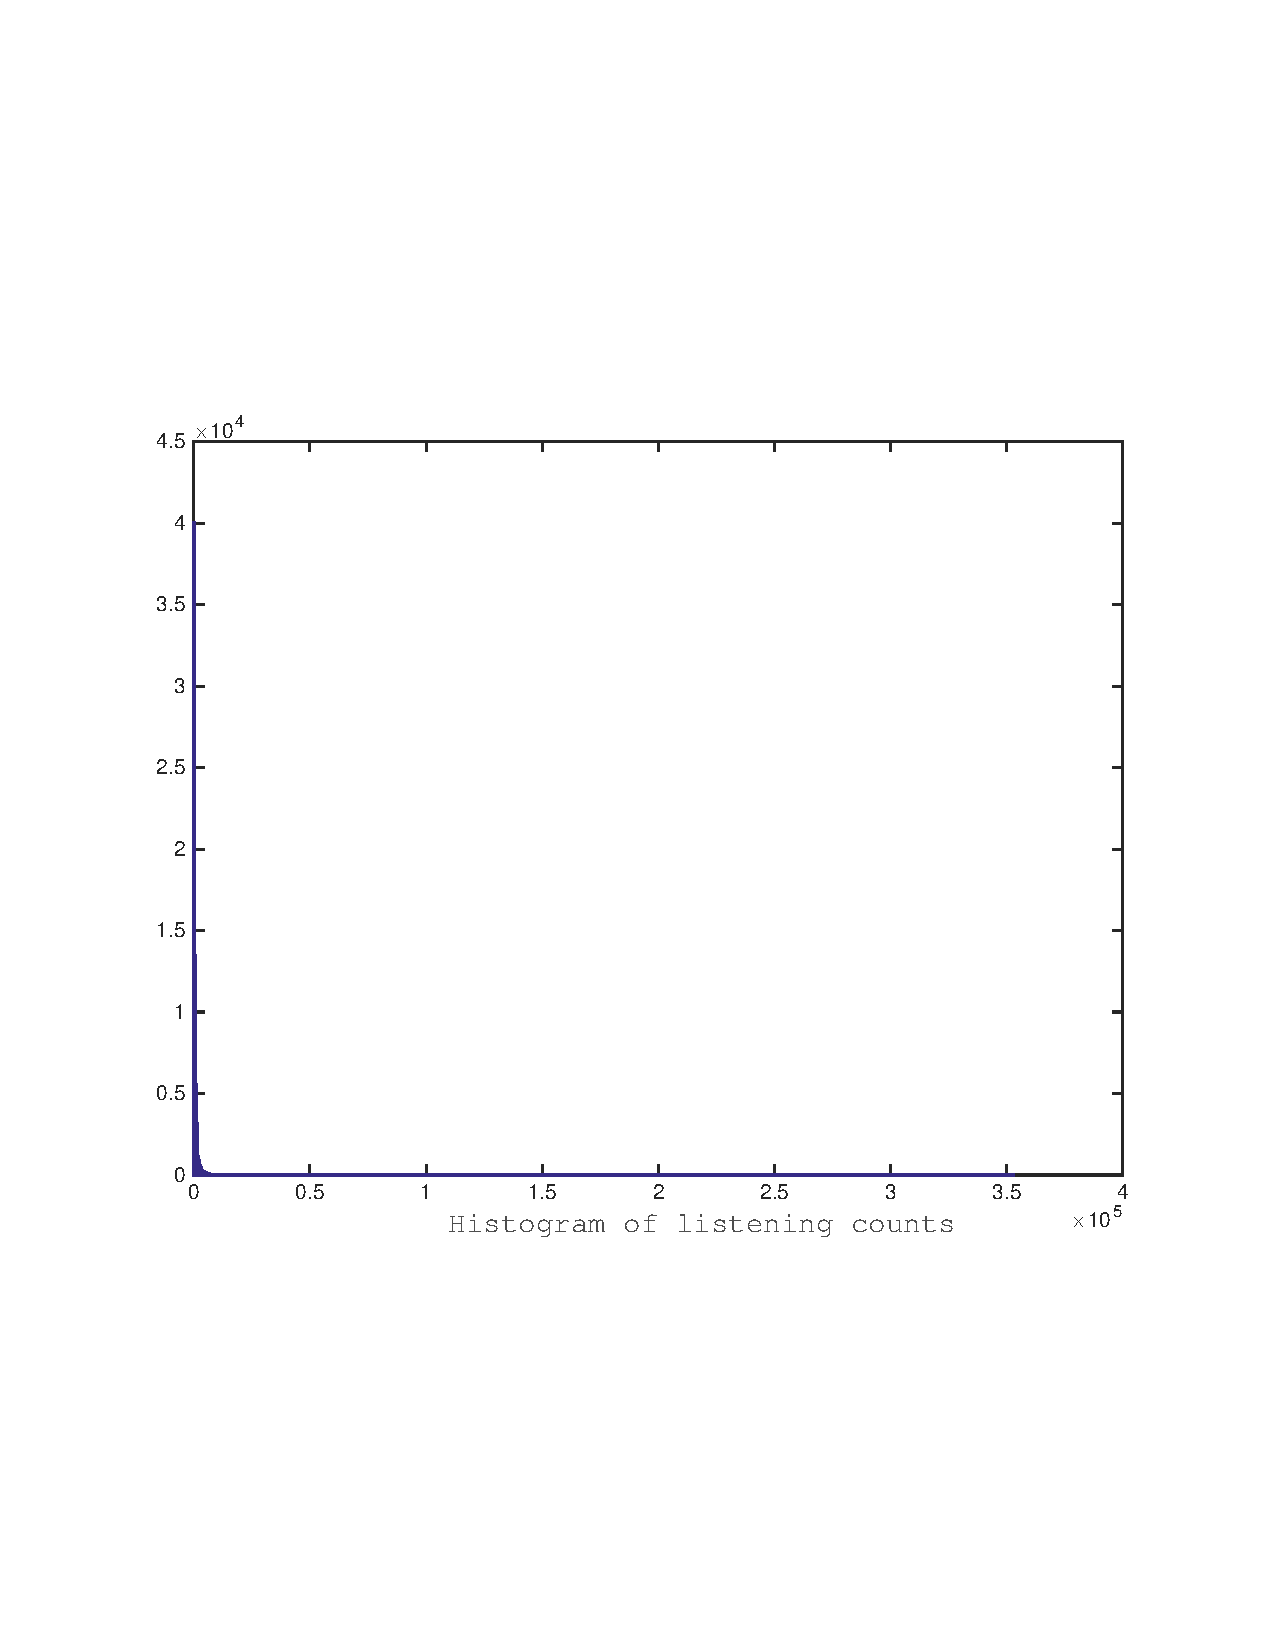
\includegraphics[width=\textwidth]{figures/histYtrain_crop.pdf}
    \caption{Before data transformation}
  \end{subfigure}
  \begin{subfigure}[b]{0.45\textwidth}
    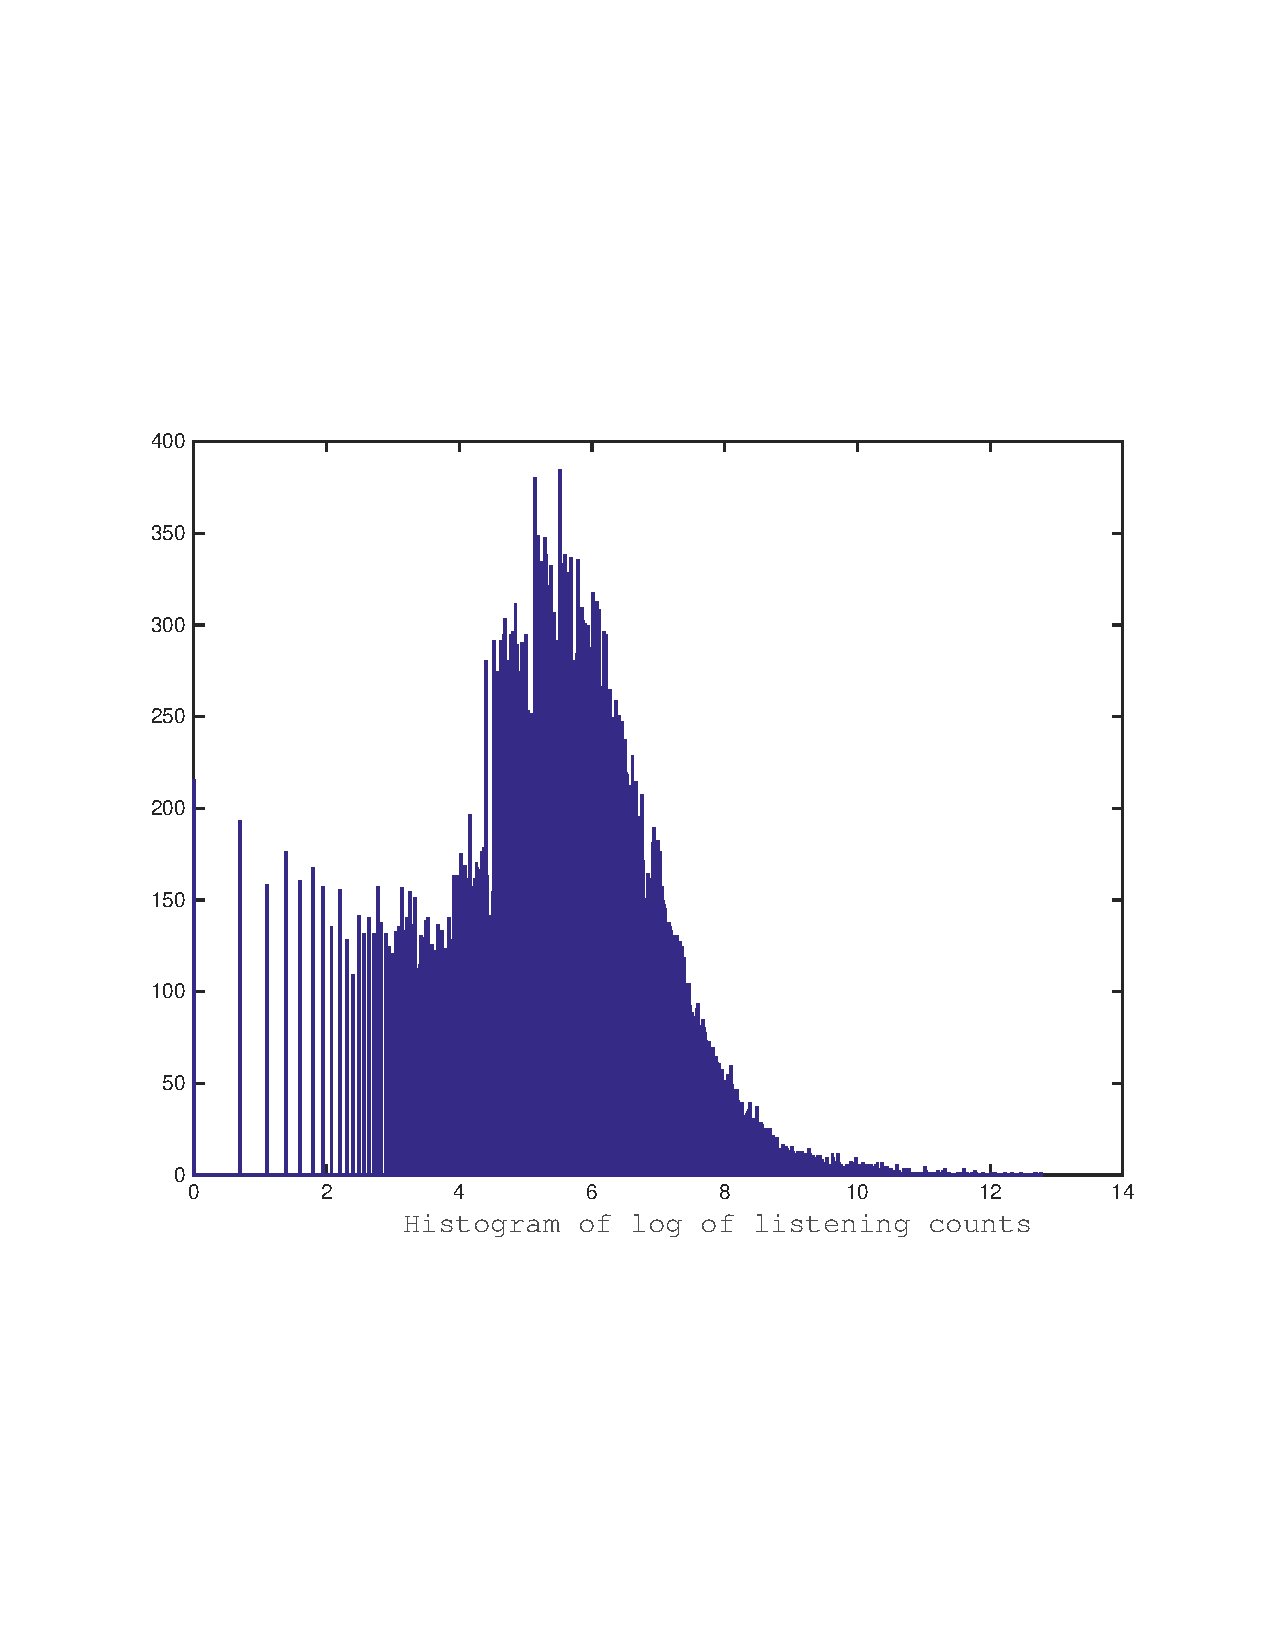
\includegraphics[width=\textwidth]{figures/histLogYtrain_crop.pdf}
    \caption{After data transformation}
  \end{subfigure}
  \caption{Distribution of listening counts}
  \label{fig:count_distribution}
\end{figure}

\begin{figure}[h]
  \centering
  \begin{subfigure}[b]{0.45\textwidth}
   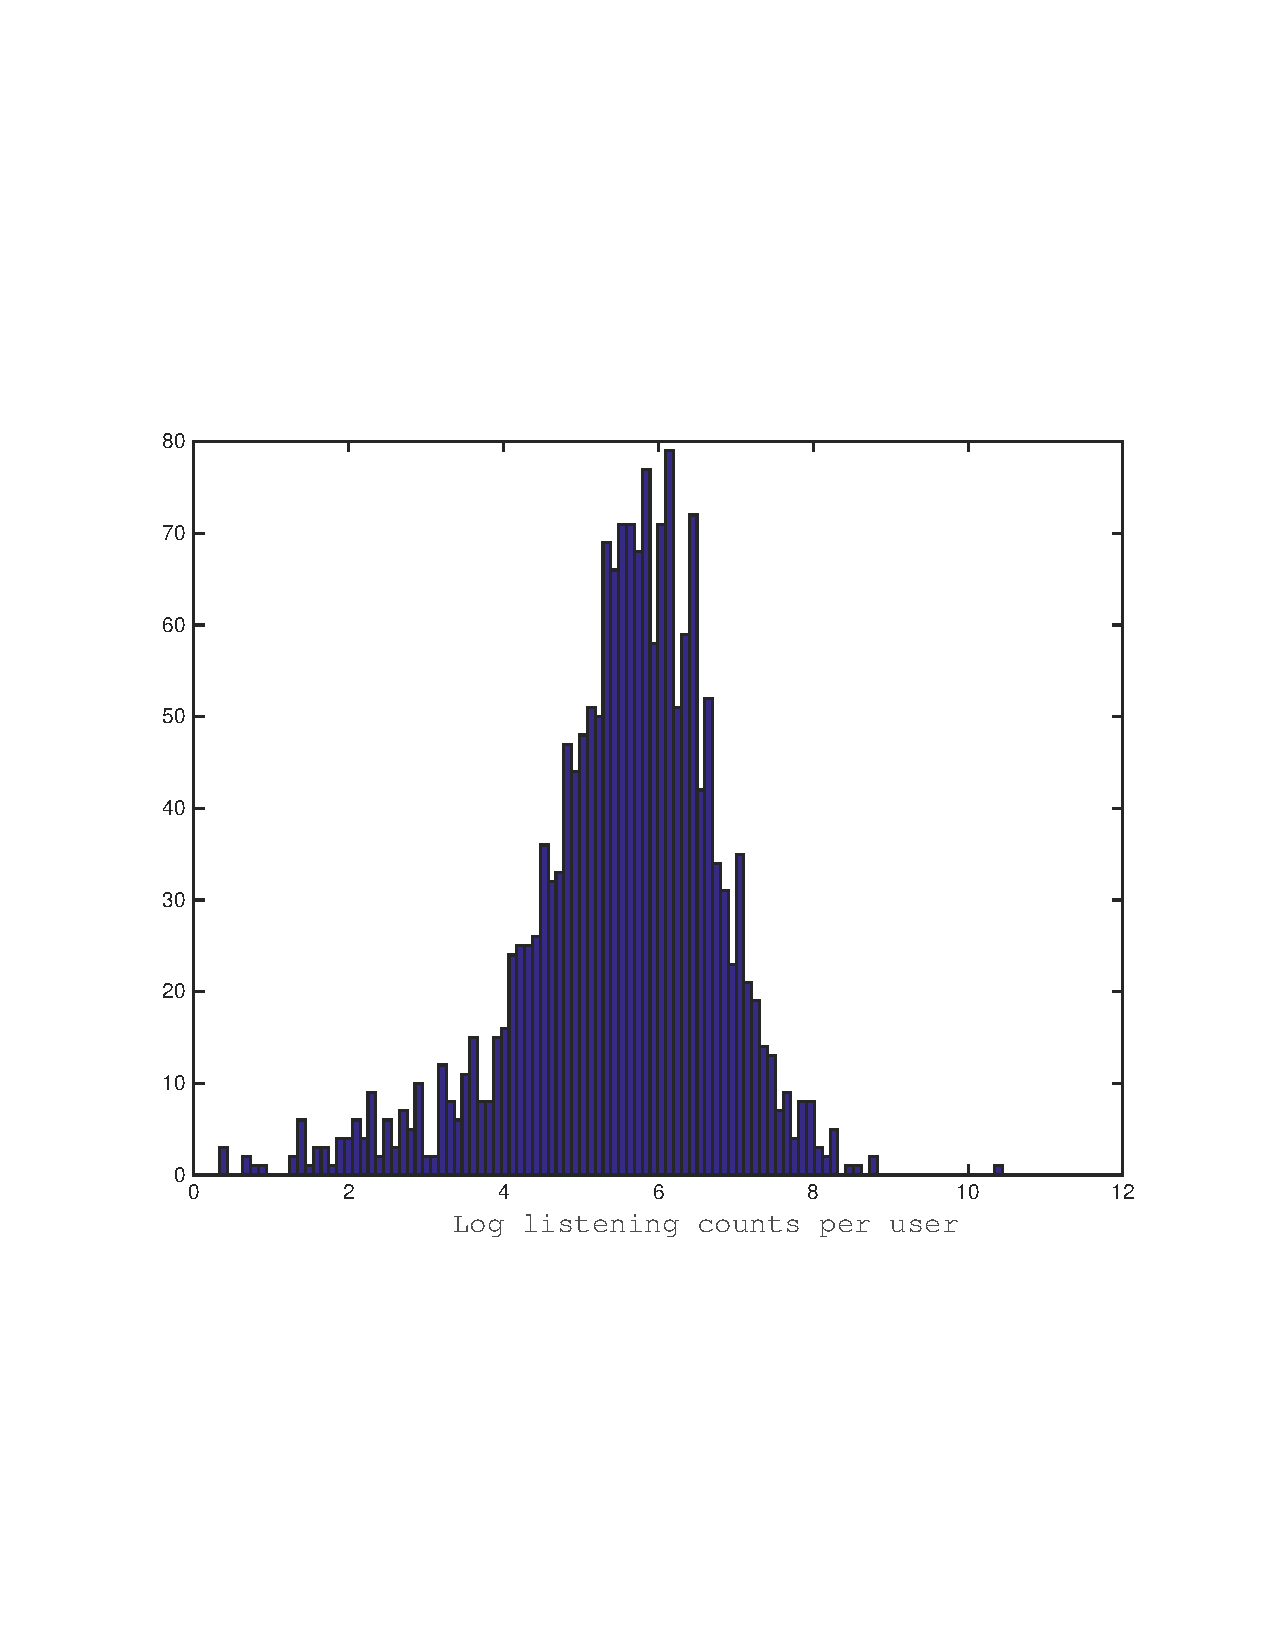
\includegraphics[width=\textwidth]{figures/histCountPerUser.pdf}
    \caption{}
  \end{subfigure}
  \begin{subfigure}[b]{0.45\textwidth}
    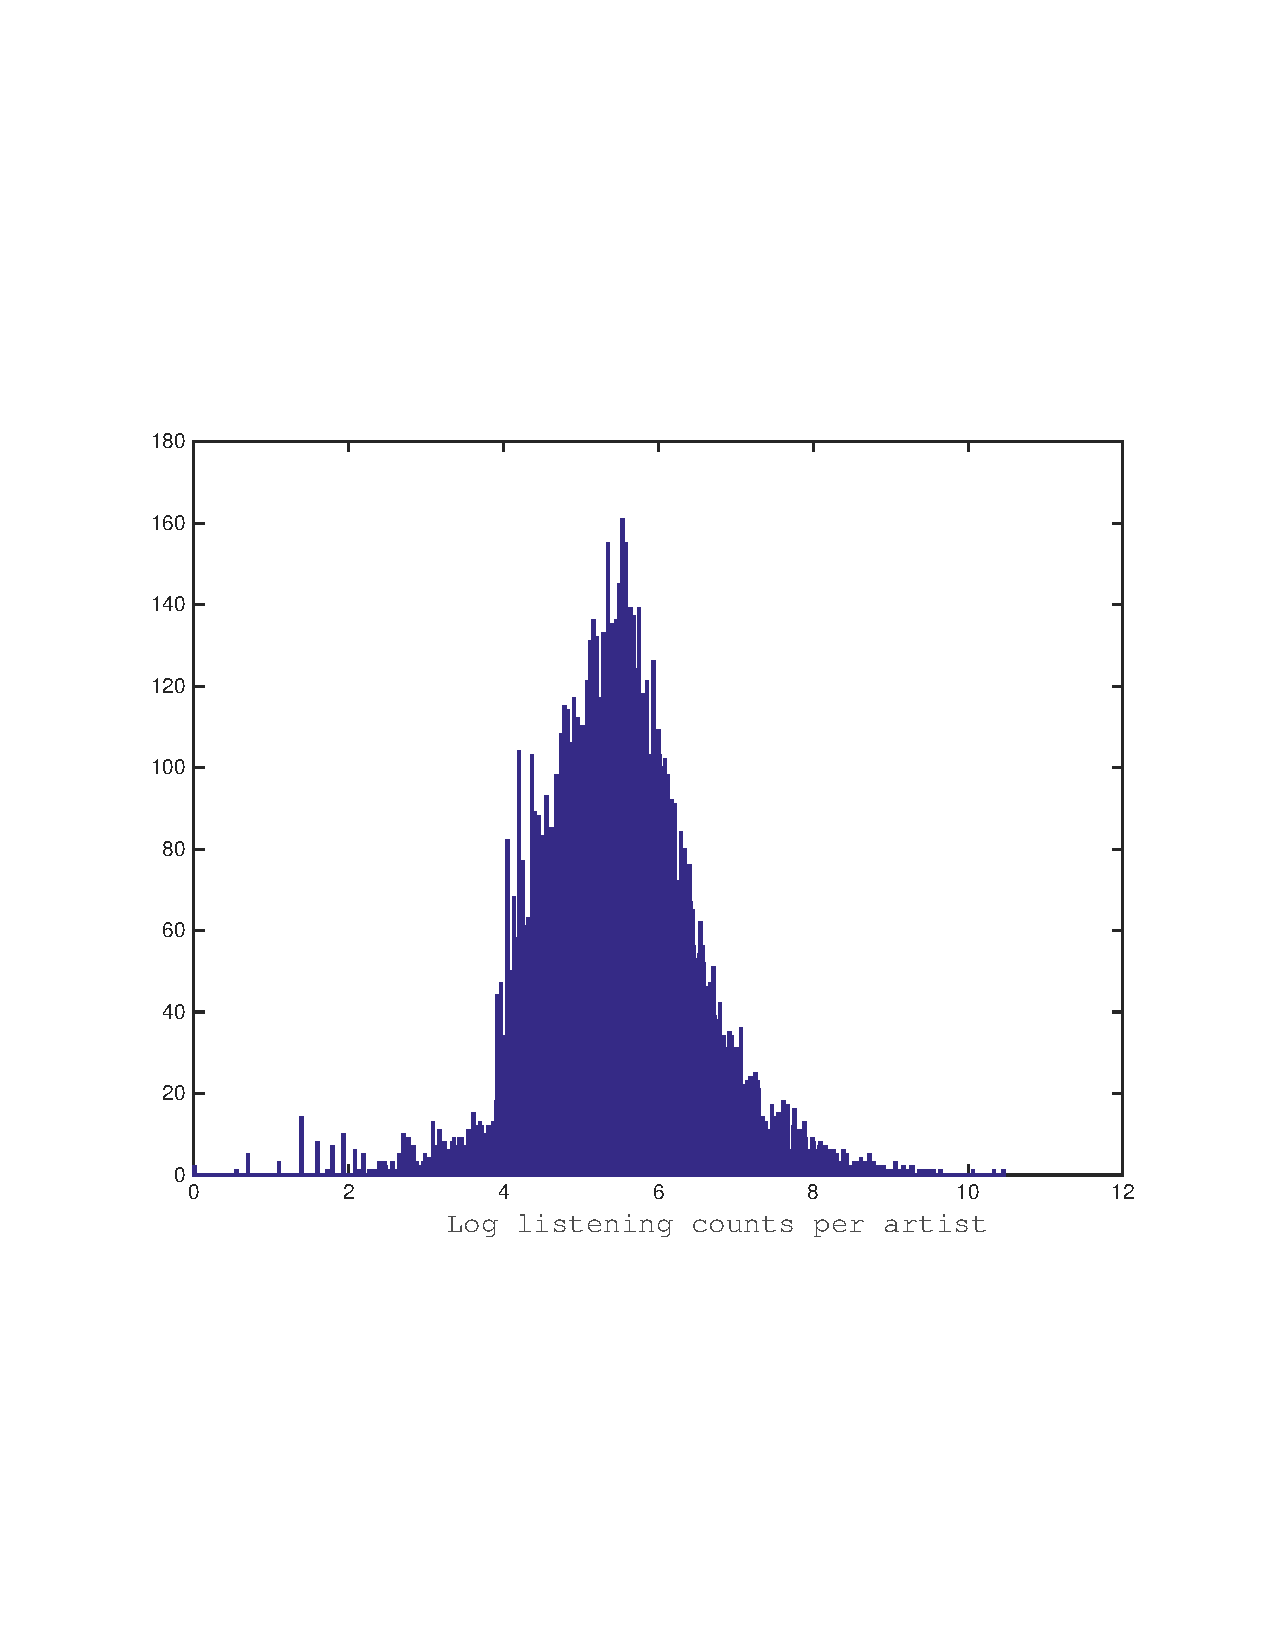
\includegraphics[width=\textwidth]{figures/histCountPerArtist.pdf}
    \caption{}
  \end{subfigure}
  \caption{Per user and per artist log of listenining count distribution}
  \label{fig:user_artist_distribution}
\end{figure}
1262 artists had 0 listening counts.

 
\subsection{Task 1}
We used 10-fold cross validation.
Splitting the data was  more difficult since we needed to make sure we do not
remove completely the counts of an user. We randomly omit for every artists 10 entries.
If an artist has less than 10 entries, nentries, then we remove nentries-1, to still have on element for testing.
\subsection{Baseline}
The mose basic prediction is to try the global average count prediction, the average count per user prediciton and average count
per artist prediction. All of these methods give similar RMSE results: 3356, 3293 and 3496 respectively.
We note that the final RMSE is composed of various values, small and large. In Fig we can see a ploto of the RMSE error terms in log format.

\subsubsection{KNN}
\subsubsection{ALS}

\subsubsection{logALS}
Using 20 clusters and $lambda in 0.01,0.1,0.5,1$ we obtain the following results using 10 fold cross validation.
\begin{center}
  \begin{tabular}{ |l | c | c| }
    \hline
     lambda & RMSE train & RMSE test \\ \hline
     0.01   & 5.0754e+09 ($\pm$  1.0793e+10) & 1.13 ($\pm$ 0.05) \\ \hline
     0.1     &  3.3508e+03 ($\pm$ 851.5037)  & 1.58 ($\pm$ 0.0608) \\ \hline
     0.5    & 3.3419e+03  ( $\pm$ 851.7858)   &13.93 ($\pm$ 0.8605)\\ \hline
     1       & 3.3876e+03 ($\pm$ 842.7349)   &25.30($\pm$ 1.48)\\ \hline
     1.5    & 3.4165e+03 ($\pm$ 837.1776) & 44.25($\pm$ 2.93) \\
    \hline
  \end{tabular}
  	\label{table:feat_transform}
    \captionof{table}{Estimated Train and Test RMSE for the two blob models.}
\end{center}
We can see that our algorithms seems to generalize better when we increase the value of
the regualization parameter. This means since we have so little data we are heavily overfitting for small values of lambda, as the train error is very small and the test error is very high. We chose our lambda to be 0.5 for the next experiments.

We varied the number of features from 10,20,30,40,50,60 with lambda = 0.5 and the results
did not improve, giving train and test RMSE of 14and 3588.
We kept the number of features to 20.

\subsubsection{Kmeans}
Inspired by the friendship graph information, we tried Kmeans with
varying values from 10 30 in steps of 5. We plot the mean train and test error using 10 fold cross validation in figure below.

We took log of the nonzeros entries of Ytrainnew and before 
computing RMSE we tranformed the data back by taking the exp
of the predicted values.
We noticed also the fact that sometimes the training error of Kmeans
(reported using exp of data) had very small fluctuations and it was not always decreasig as the algorithm convergence properties would expect. This is due to the fact that Kmeans miminizes squared error but our cost is a little different since we transform the data using exp.

We had avary large variations in the algorithm's output.

One reason for performing Kmeans for clusteringover users 
instead of over artists, although the number of artists is larger than the number of users is to be easier in Task 2.



We can see that our algorithm performs for

\subsection{Task 2}
\subsubsection{Friendship information}
Regarding the friendshiop information, we noticed there are 22 connected components, but many of them contained.
1776 nodes and 22904 edges.
Using Vincent D Blondel, Jean-Loup Guillaume, Renaud Lambiotte, Etienne Lefebvre, Fast unfolding of communities in large networks, in Journal of Statistical Mechanics: Theory and Experiment 2008 (10), P1000 and the Gephi tool to find properties of the graph, it suggested it has about
32 communities, of which 8 had more than 150 members and the others being very small. (22 connected components, of which 20 are very small < 50 users.) This was run to give us an idea of the number of clusters we could use in Kmeans.

\subsection{•}
In this task we are given a set of new users and their friendship information.
The task is to predict their listening counts based only on their friendship information with
people for which we already have some information about their listening habbits.
We experiment with three methods.
 A baseline method in which a (user,artist) count is predicted
using the average count of its friends, global average if that informatino id not present.

The second method uses the 20 clusters from the previous method and predicts the count
as an average weight of the listening counts of the clusters of the friends.

The thirs method uses the 20 clusters from the previous method in a weighted average approach but this time also the friends of the friends information is used. 

\subsection{Summary}



